\documentclass[10pt,a4paper]{article}
\usepackage[utf8]{inputenc}
\usepackage{graphicx}
\def\Pr{\mathop{\rm Pr}}
\usepackage[landscape,margin=1cm]{geometry}
\usepackage[english]{babel}
\usepackage{tikz}
\usetikzlibrary{arrows,snakes,backgrounds,shapes.geometric}
\title{Neuromatch Academy Pre-Requisite Refresher - Summary Sheet}
\author{Neuromatch}
%\date{July 2019}
\usepackage[default]{raleway}
\usepackage{fontawesome}
\usepackage[T1]{fontenc}

\usepackage{hyperref}
\usepackage{enumitem}
\usepackage{lipsum}

\usepackage{xcolor}
\definecolor{customcolor}{HTML}{616AC5}
\definecolor{alert}{HTML}{CD5C5C}
\definecolor{w3schools}{HTML}{4CAF50}
\definecolor{subbox}{gray}{0.60}
\definecolor{codecolor}{HTML}{FFC300}
\colorlet{xx}{customcolor}


%--------------------------Editor mode.

\usepackage
[citestyle=authoryear,
sorting=nty,	  		%Sorts bibliography by year, name, title
autocite=footnote, 		%Autocite command generates footnotes
autolang=hyphen, 		
mincrossrefs=1, 	
backend=biber]
{biblatex}

\DeclareFieldFormat{postnote}{#1}
\DeclareFieldFormat{multipostnote}{#1}
\DeclareAutoCiteCommand{footnote}[f]{\footcite}{\footcites}

\bibliography{literature}
%----------------------------------------
%--------------------------------------------------------------------------------
\usepackage{tcolorbox}

\tcbuselibrary{most,listingsutf8,minted}

\tcbset{tcbox width=auto,left=1mm,top=1mm,bottom=1mm,
right=1mm,boxsep=1mm,middle=1pt}

\newenvironment{mycolorbox}[2]{%
\begin{tcolorbox}[grow to left by=-1em,grow to right by=-1em,capture=minipage,fonttitle=\large\bfseries, enhanced jigsaw,boxsep=1mm,colback=#1!30!white,on line,tcbox width=auto, toptitle=0mm,colframe=#2,opacityback=0.7,nobeforeafter,title=#2]%
}{\end{tcolorbox}\\[0.2em]}

\newenvironment{subbox}[2]{%
\begin{tcolorbox}[capture=minipage,fonttitle=\normalsize\bfseries, enhanced jigsaw,boxsep=1mm,colback=#1!30!white,on line,tcbox width=auto,left=0.3em,top=1mm, toptitle=0mm,colframe=#1,opacityback=0.7,nobeforeafter,title=#2]\footnotesize %
}{\normalsize\end{tcolorbox}\vspace{0.1em}}

\newenvironment{multibox}[1]{%
\begin{tcbraster}[raster columns=#1,raster equal height,nobeforeafter,raster column skip=1em,raster left skip=1em,raster right skip=1em]}{\end{tcbraster}}

\newenvironment{textbox}[1]{\begin{mycolorbox}{customcolor}{#1}}{\end{mycolorbox}}

%-------------------------------
\newtcblisting{codebox}[2]{colback=codecolor!5,colframe=codecolor!80!black,listing only, 
minted options={numbers=left,style=tcblatex,fontsize=\normalsize,breaklines,autogobble,linenos,numbersep=1mm},
left=5mm,enhanced,
title=#2, fonttitle=\bfseries,
listing engine=minted,minted language=#1}

%--------------------------------------------------------------------------------
\newcommand{\punkti}{~\lbrack\dots\rbrack~}

\renewenvironment{quote}
               {\list{\faQuoteLeft\phantom{ }}{\rightmargin\leftmargin}%
                \item\relax\scriptsize\ignorespaces}
               {\unskip\unskip\phantom{xx}\faQuoteRight\endlist}
               

%--------------------------------------------------------------------------------
\newcommand{\bgupper}[3]{\colorbox{#1}{\color{#2}\huge\bfseries\MakeUppercase{#3}}}
\newcommand{\bg}[3]{\colorbox{#1}{\bfseries\color{#2}#3}}

\newcommand{\mycommand}[2]{{\ttfamily\detokenize{#1}}~\dotfill{}~{\footnotesize #2}\\}
\newcommand{\sep}{{\scriptsize~\faCircle{ }~}}


\newcommand{\bggreen}[1]{\medskip\bgupper{w3schools}{black}{#1}\\[0.5em]}
\newcommand{\green}[1]{\smallskip\bg{w3schools}{white}{#1}\\}
\newcommand{\red}[1]{\smallskip\bg{alert}{white}{#1}\\}

\usepackage{multicol}
\setlength{\columnsep}{30pt}

\setlength{\parindent}{0pt}
\pagestyle{empty}

\usepackage{csquotes}

\newcommand{\loremipsum}{Lorem ipsum dolor sit amet.}

\clearpage

%--------------------------------------------------------------------------------
\begin{document}


%\section{Data Type}

\includegraphics[scale=0.1]{Figures/nma-logo-square-4xp.jpeg}\href{https://compneuro.neuromatch.io/tutorials/intro.html}{\textbf{\Huge{Neuromatch Academy Pre-Requisite Refresher - Summary Sheet}}\footnote{’t Hart et al., (2022). Neuromatch Academy: a 3-week, online summer school in computational neuroscience. Journal of Open Source Education, 5(49), 118. https://doi.org/10.21105/jose.00118}}
%$\subsection*{Cheat Sheet}
\small
\begin{multicols}{3}
%\scriptsize
\let\clearpage\relax
\begin{textbox}{\href{https://compneuro.neuromatch.io/tutorials/W0D3_LinearAlgebra/student/W0D3_Tutorial1.html}{Vectors (W0D3T1)} }
\begin{subbox}{subbox}{A Vector}
\scriptsize
A vector, $\mathbf{v}$, is a short hand way of representing a list of numbers like $x$ and $y$ coordinates:
\begin{equation}
\mathbf{v} = 
\begin{bmatrix}
4 \\
1
\end{bmatrix},
\end{equation}

A 2-D vector $\mathbf{v}$ has a direction and a length. A normalized vector $\widetilde{\mathbf{v}}$ has a length 1.

\centering
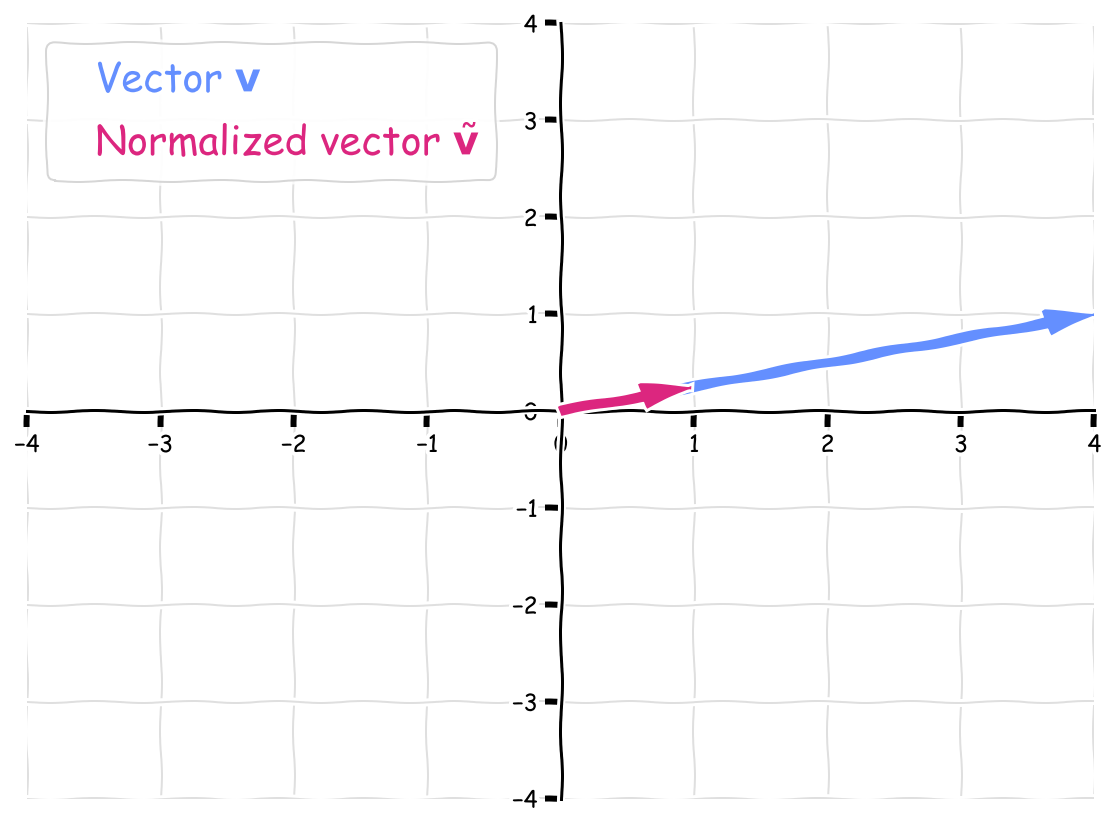
\includegraphics[scale=0.1]{Figures/PreCourse/Figure1.png}
\end{subbox}

\begin{subbox}{subbox}{Linear Combination of Vectors}
\scriptsize
Two vectors $\mathbf{x}$ and $\mathbf{y}$ can be added together and multiplied by parameters $a$ and $b$ to get a new vector $\mathbf{z}$
\begin{equation}
\mathbf{z} = a\mathbf{x} + b\mathbf{y}
\end{equation}

given $\mathbf{x} = \begin{bmatrix}3 \\ 1 \end{bmatrix}$ and $\mathbf{y} = \begin{bmatrix}-1 \\ 2 \end{bmatrix}$, and $a=-1$ and $b=2$
\begin{equation*}
\begin{bmatrix}-6 \\ 3 \end{bmatrix}= -1\begin{bmatrix}3 \\ 1 \end{bmatrix} +2 \begin{bmatrix}-1 \\ 2 \end{bmatrix}.
\end{equation*}
\centering
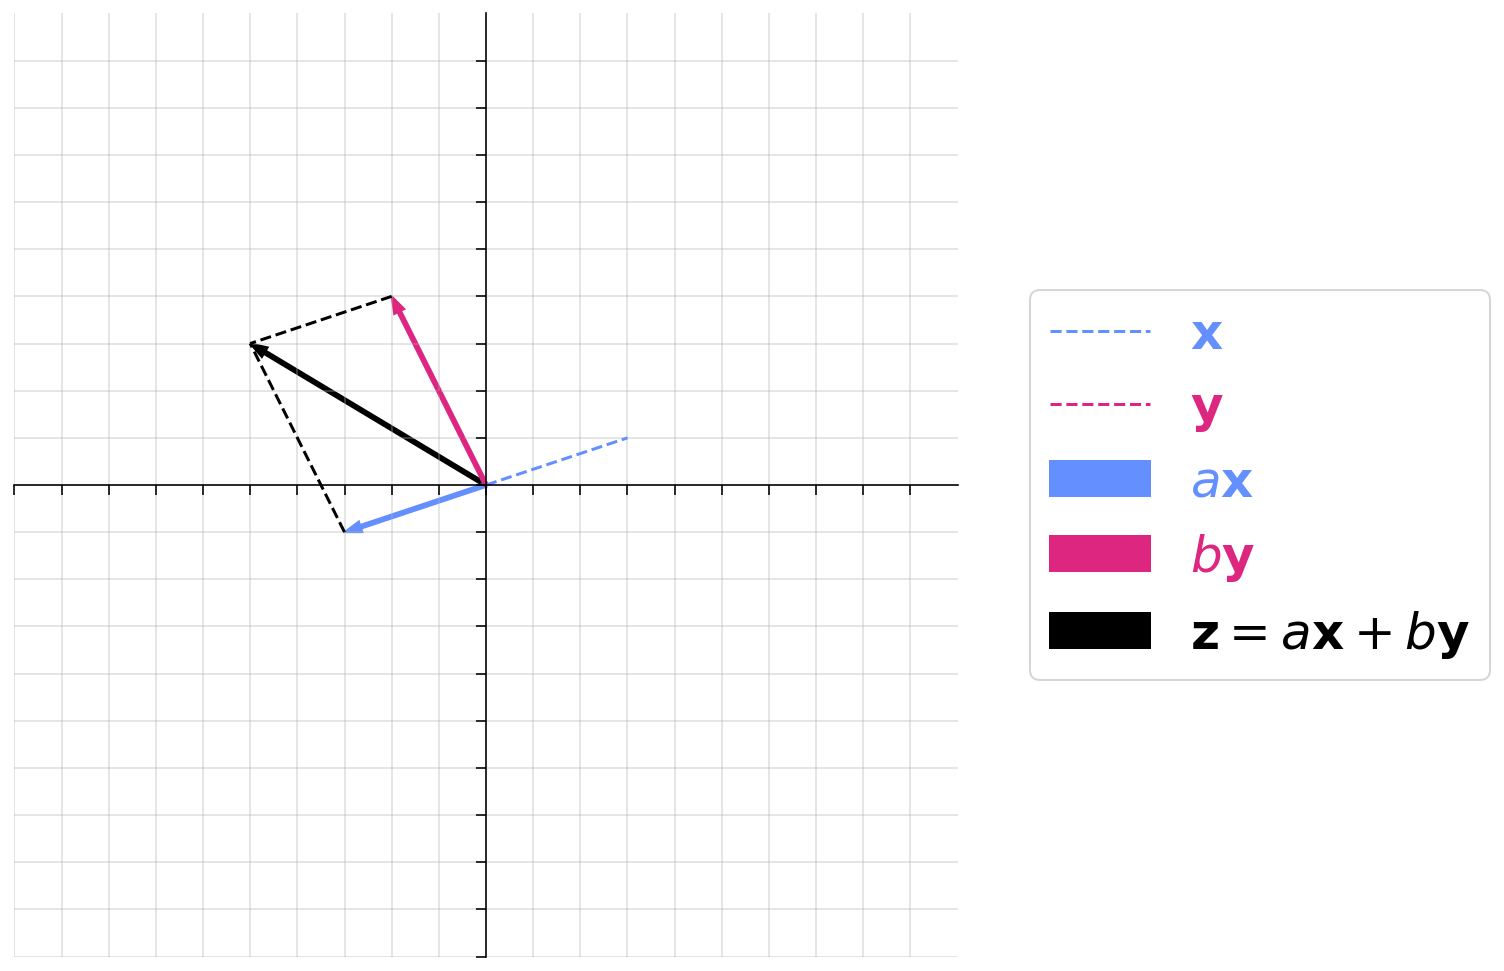
\includegraphics[scale=0.15]{Figures/PreCourse/Figure3.png}
\end{subbox}
\begin{subbox}{subbox}{The Geometry of the Dot Product $\mathbf{w}\cdot\mathbf{r}$}
\scriptsize
An alternate way of defining the dot product is as the multiple of the lengths of the two vectors and the angle between them $\theta$:

\begin{equation}
\mathbf{x} \cdot \mathbf{y} = ||\mathbf{x}|| \cdot ||\mathbf{y}|| \cdot \cos(\theta).
\end{equation}

\end{subbox}
\end{textbox}
%%%%%%%%%%%%%%%%%%%%%%%%%%%%%%%%%%%%%%%%%%%%%%%%%%
\begin{textbox}{Vectors (W0D3T1) }
\begin{subbox}{subbox}{Dot Product $\mathbf{w}\cdot\mathbf{r}$}
\scriptsize
Given two retinal neurons with varying firing rates ($r_1$ and $r_2$).  The retinal firing rates can be represented as the vector $\mathbf{r} = \begin{bmatrix} r_1\\ r_2\\ \end{bmatrix}$.

The weights from each of these to an LGN neuron. The weights are represented with the vector $\mathbf{w} = \begin{bmatrix} w_1\\ w_2\\ \end{bmatrix}$.

The LGN firing rate is the dot product of the retinal firing rate vector and the weight vector:
\begin{equation}
g = \mathbf{w}\cdot\mathbf{r} = w_1r_1 + w_2r_2
\end{equation}

\centering
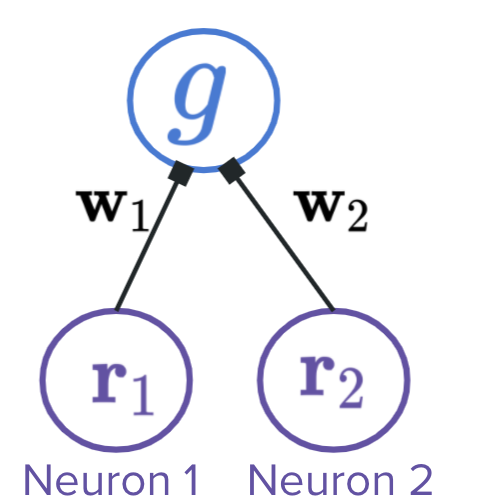
\includegraphics[scale=0.3]{Figures/PreCourse/Figure2.png}
\end{subbox}

\end{textbox}
%%%%%%%%%%%%%%%%%%%%%%%%% 
%%%%%%%%%%%%%%%%%%%%%%%%%
\begin{textbox}{Matrices (W0D3T2)  }
\begin{subbox}{subbox}{Intro to Matrices}
\scriptsize
We will look at a group of 2 LGN neurons which get input from 2 retinal neurons: we will call the population of LGN neurons population $p$. Below, we have the system of linear equations that dictates the neuron models for each population. $r_1$ and $r_2$ correspond to the retinal neural activities (of neuron 1 and 2). $g_{p_1}$ and  $g_{p_2}$ correspond to the responses of the LGN neurons 1 and 2 in population $p$. 

\begin{align}
r_1 + 3r_2 &= g_{p_1} \\
2r_1 + r_2 &= g_{p_2} 
\end{align}
Cast each equation (i.e., $g_{p_1}$ and $g_{p_2}$) as a matrix-vector multiplication: 

\begin{equation}
\mathbf{g}_p = \mathbf{P}\mathbf{r}
\end{equation}

where \begin{equation}\mathbf{P}=
\begin{bmatrix}
1 & 3 \\
2 & 1
\end{bmatrix}
\end{equation}

is the weight matrix to population $p$. 
\end{subbox}
\end{textbox}
\begin{textbox}{Matrices (W0D3T2)}

\begin{subbox}{subbox}{Matrices as Linear Transformations}
\scriptsize
Matrices can be thought of as enacting linear transformations. When multiplied with a vector, they transform it into another vector. In fact, they are transforming a grid of space in a linear manner: the origin stays in place and grid lines remain straight, parallel, and evenly spaced.

\centering
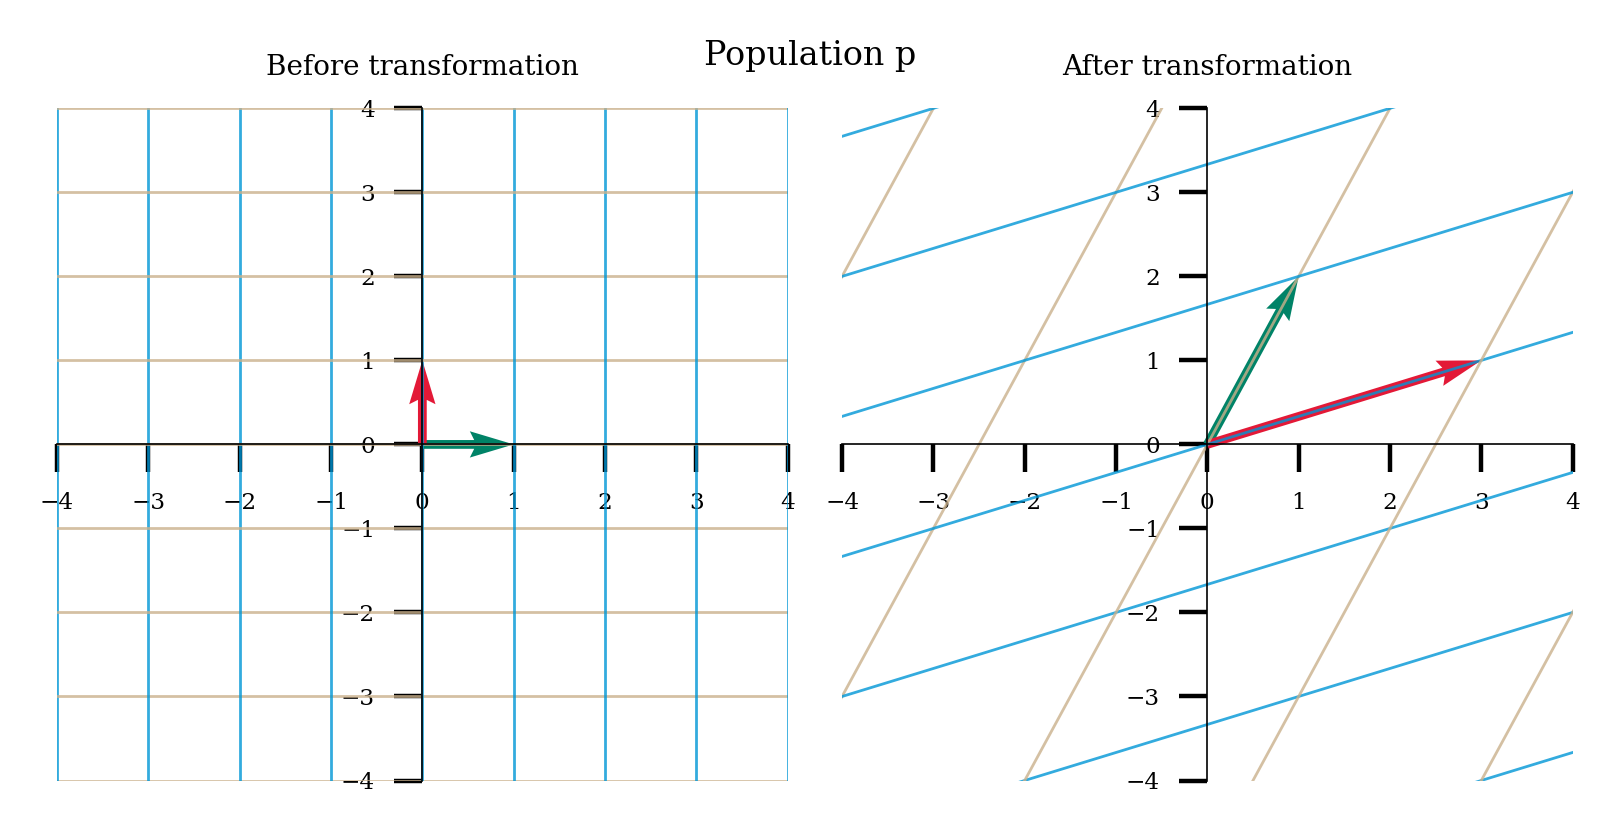
\includegraphics[scale=0.5]{Figures/PreCourse/Figure4.png}
\end{subbox}


\begin{subbox}{subbox}{Eigenvalues \& Eigenvectors}
\tiny
Eigenvectors, $\mathbf{v}$ of a matrix $\mathbf{W}$ are vectors that, when multipled by the matrix, equal a scalar multiple of themselves. That scalar multiple is the corresponding eigenvalue, $\lambda$.

\begin{equation}
\mathbf{W}\mathbf{v} = \lambda\mathbf{v}
\end{equation}

If we have one eigenvector for a matrix, we technically have an infinite amount: every vector along the span of that eigenvector is also an eigenvector. So, we often use the unit vector in that direction to summarize all the eigenvectors along that line. 

Just by looking at eigenvectors before and after a transformation, can you describe what the transformation is in words? Try for each of the two plots below.

\centering
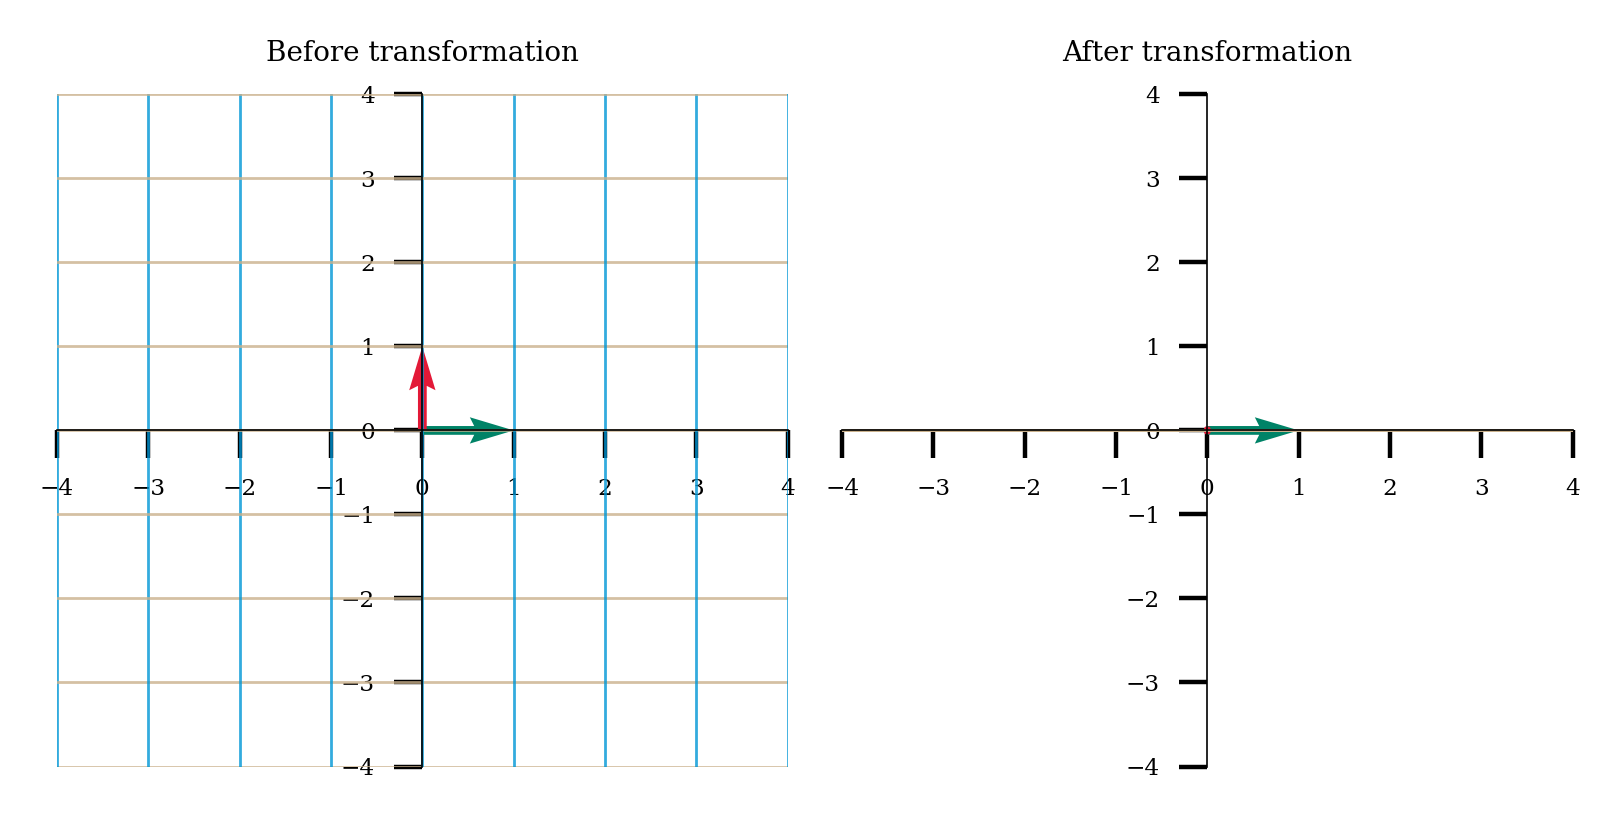
\includegraphics[scale=0.1]{Figures/PreCourse/Figure5.png}

\end{subbox}

\begin{subbox}{subbox}{Matrix Multiplication}
\tiny
We sometimes want to multiple two matrices together, instead of a matrix with a vector. Let's say we're multiplying matrices $\mathbf{A}$ and $\mathbf{B}$ to get $\mathbf{C}$:
\begin{equation}
\mathbf{C} = \mathbf{A}\mathbf{B}\text{.}
\end{equation}

We take the dot product of each row of A with each column of B. The resulting scalar is placed in the element of $\mathbf{C}$ that is the same row (as the row in A) and column (as the column in B). So the element of $\mathbf{C}$ at row 4 and column 2 is the dot product of the 4th row of $\mathbf{A}$ and the 2nd column of $\mathbf{B}$. We can write this in a formula as:
\begin{equation}\mathbf{C}_{\text{row i, column j}} = \mathbf{A}_{\text{row i}} \cdot \mathbf{B}_{\text{column j}}
\end{equation}
\end{subbox}
\end{textbox}

\clearpage
\clearpage
\begin{textbox}{\href{https://compneuro.neuromatch.io/tutorials/W0D4_Calculus/student/W0D4_Tutorial1.html}{Calculus (W0D4T1)} - Differentiation and Integration}
\begin{subbox}{subbox}{Introduction}
\scriptsize
\textbf{Differentiation} of a function $f(t)$ gives you the derivative of that function \begin{equation} \frac{d(f(t))}{dt}.
\end{equation} A derivative captures how sensitive a function is to slight changes in the input for different ranges of inputs. 

\textbf{Integration} can be thought of as the reverse of differentiation
\begin{equation}
\int f(t)dt.
\end{equation}
\centering
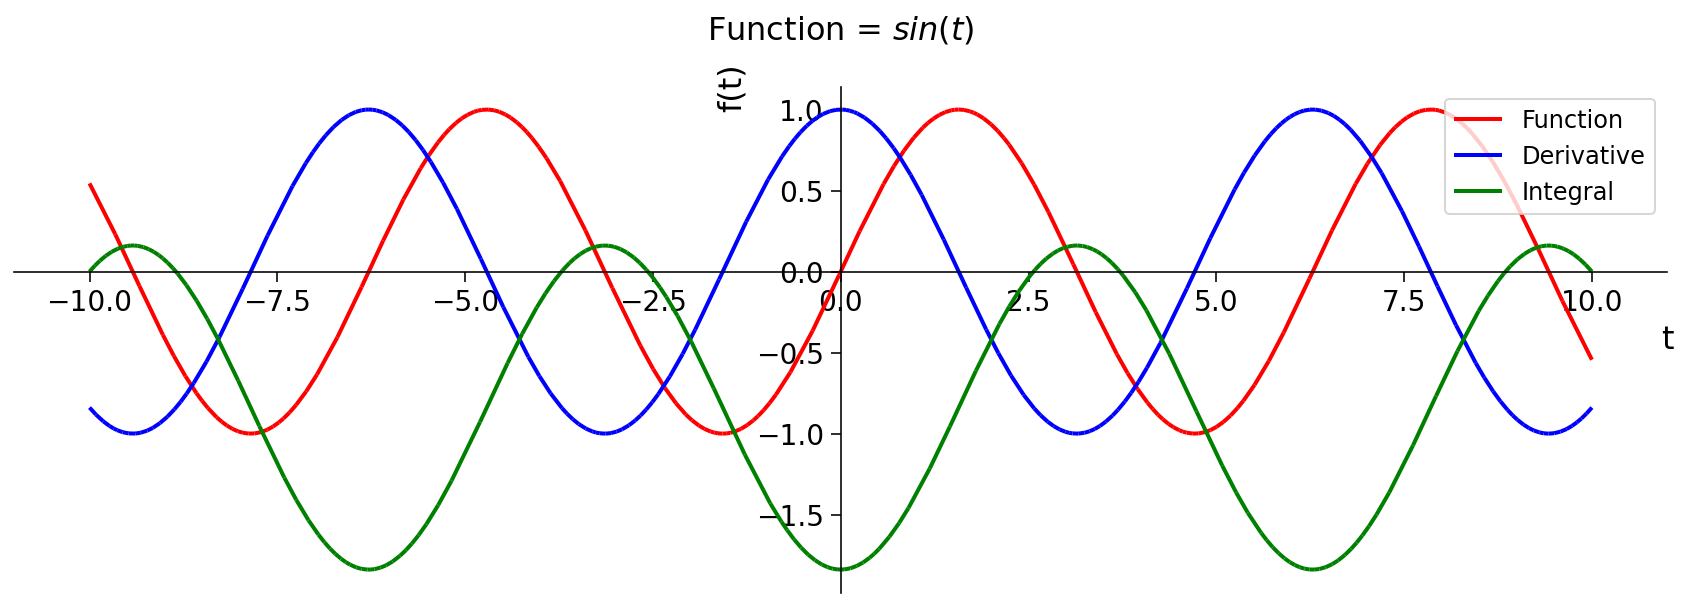
\includegraphics[scale=0.2]{Figures/PreCourse/CFigure1.png}
\end{subbox}

\begin{subbox}{subbox}{Analytical Differentiation}
\scriptsize{
When we find the derivative analytically, we are finding the exact formula for the derivative function. 
To do this, instead of having to do some fancy math every time, we can consult a list of common derivatives such as:

\textbf{ \href{https://en.wikipedia.org/wiki/Product_rule}{The Product Rule}}
\begin{align}
f(t) &= u(t)\cdot v(t) \\
\frac{d(f(t))}{dt} &= v\cdot \frac{du}{dt} + u\cdot \frac{dv}{dt}
\end{align}
\textbf{\href{https://en.wikipedia.org/wiki/Chain_rule}{The Chain Rule}:}
\begin{equation}
\frac{dr}{da} = \frac{dr}{dt}\cdot\frac{dt}{da}.
\end{equation}
}
\end{subbox}
\begin{subbox}{subbox}{Numerical Differentiation}
\scriptsize{Formally, the derivative of a function $f(x)$ at any value $a$ is given by the finite difference formula (FD): 
\begin{equation}
FD = \frac{f(a+h) - f(a)}{h}
\end{equation}
As $h\rightarrow 0$, the FD approaches the actual value of the derivative.}

\centering
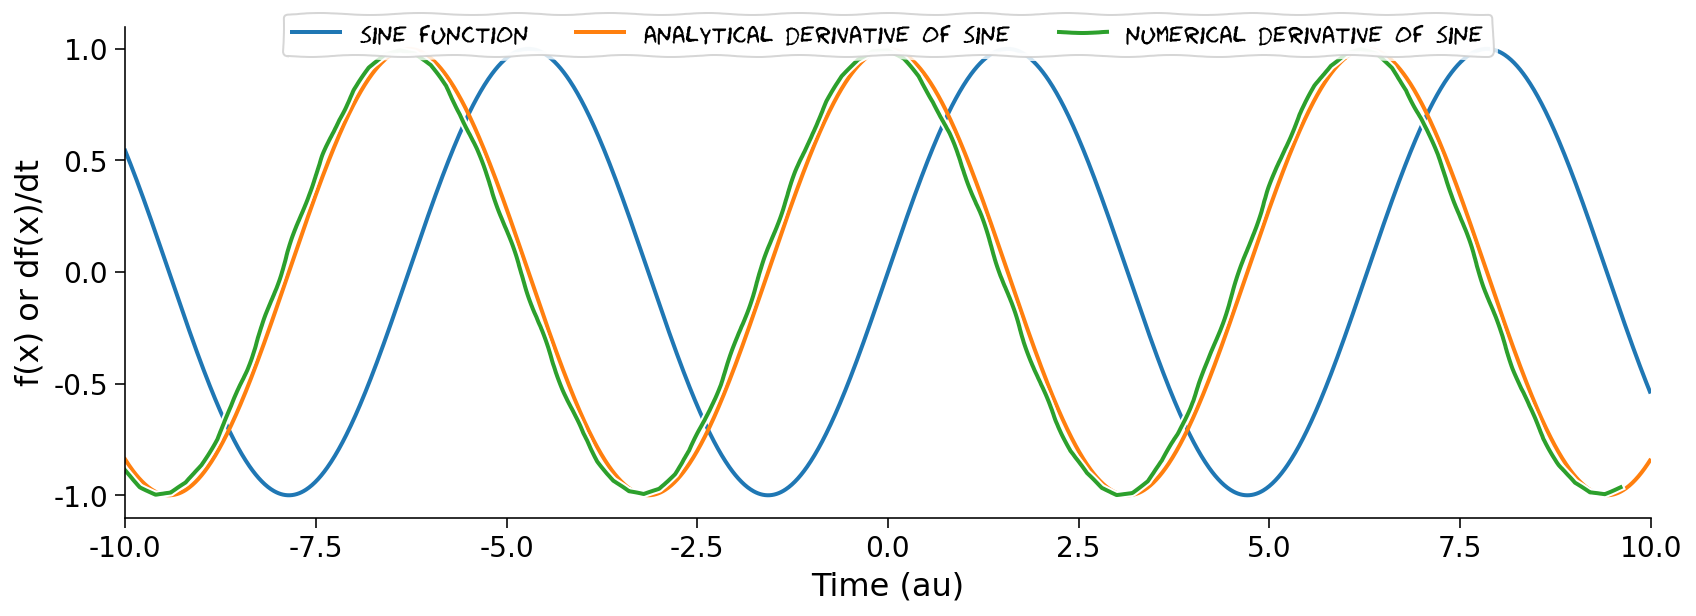
\includegraphics[scale=0.2]{Figures/PreCourse/CFigure2.png}
\end{subbox}
\end{textbox}
%%%%%%%%%%%%%%%%%%%%%%%%%%%%%%%%%%%%%%%%%%%%%%%%%%
\begin{textbox}{Calculus (W0D4T1) - Differentiation and Integration}
%%%%%%%%%%%%%%%
\begin{subbox}{subbox}{Functions of Multiple Variables}
\scriptsize
In most cases, we encounter functions of multiple variables. For example, in the brain, the firing rate of a neuron is a function of both excitatory and inhibitory input rates. In the following, we will look into how to calculate derivatives of such functions.

When we take the derivative of a multivariable function with respect to one of the variables it is called the **partial derivative**. For example if we have a function:

\begin{align}
f(x,y) = x^3  +2xy+ y^2
\end{align}

The we can define the partial derivatives as

\begin{align}
\frac{\partial(f(x,y))}{\partial x} = 3x^2  +2y+ 0 \\
\frac{\partial(f(x,y))}{\partial y} = 0+ 2x+2y
\end{align}
\centering
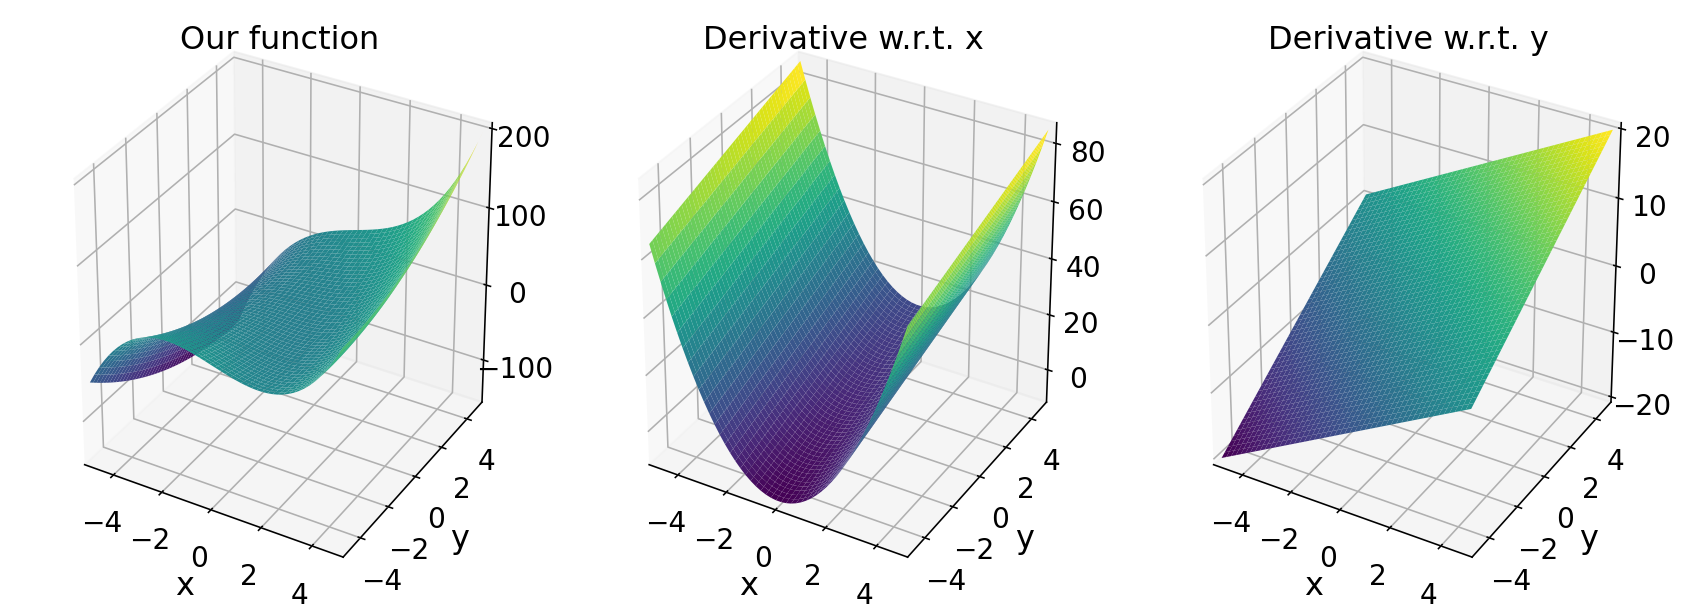
\includegraphics[scale=0.2]{Figures/PreCourse/CFigure3.png}

\end{subbox}
\begin{subbox}{subbox}{Numerical Integration (Riemann Sum)}
\scriptsize

Geometrically, integration is the area under the curve. This interpretation gives two formal ways to calculate the integral of a function numerically. 

If we wish to integrate a function $f(t)$ with respect to $t$, then first we divide the function into $n$ intervals of size $dt = a-b$, where $a$ is the starting of the interval. Thus, each interval gives a rectangle with height $f(a)$ and width $dt$. By summing the area of all the rectangles, we can approximate the area under the curve. As the size $dt$ approaches to zero, our estimate of the integral approaches the analytical calculation. 

\centering
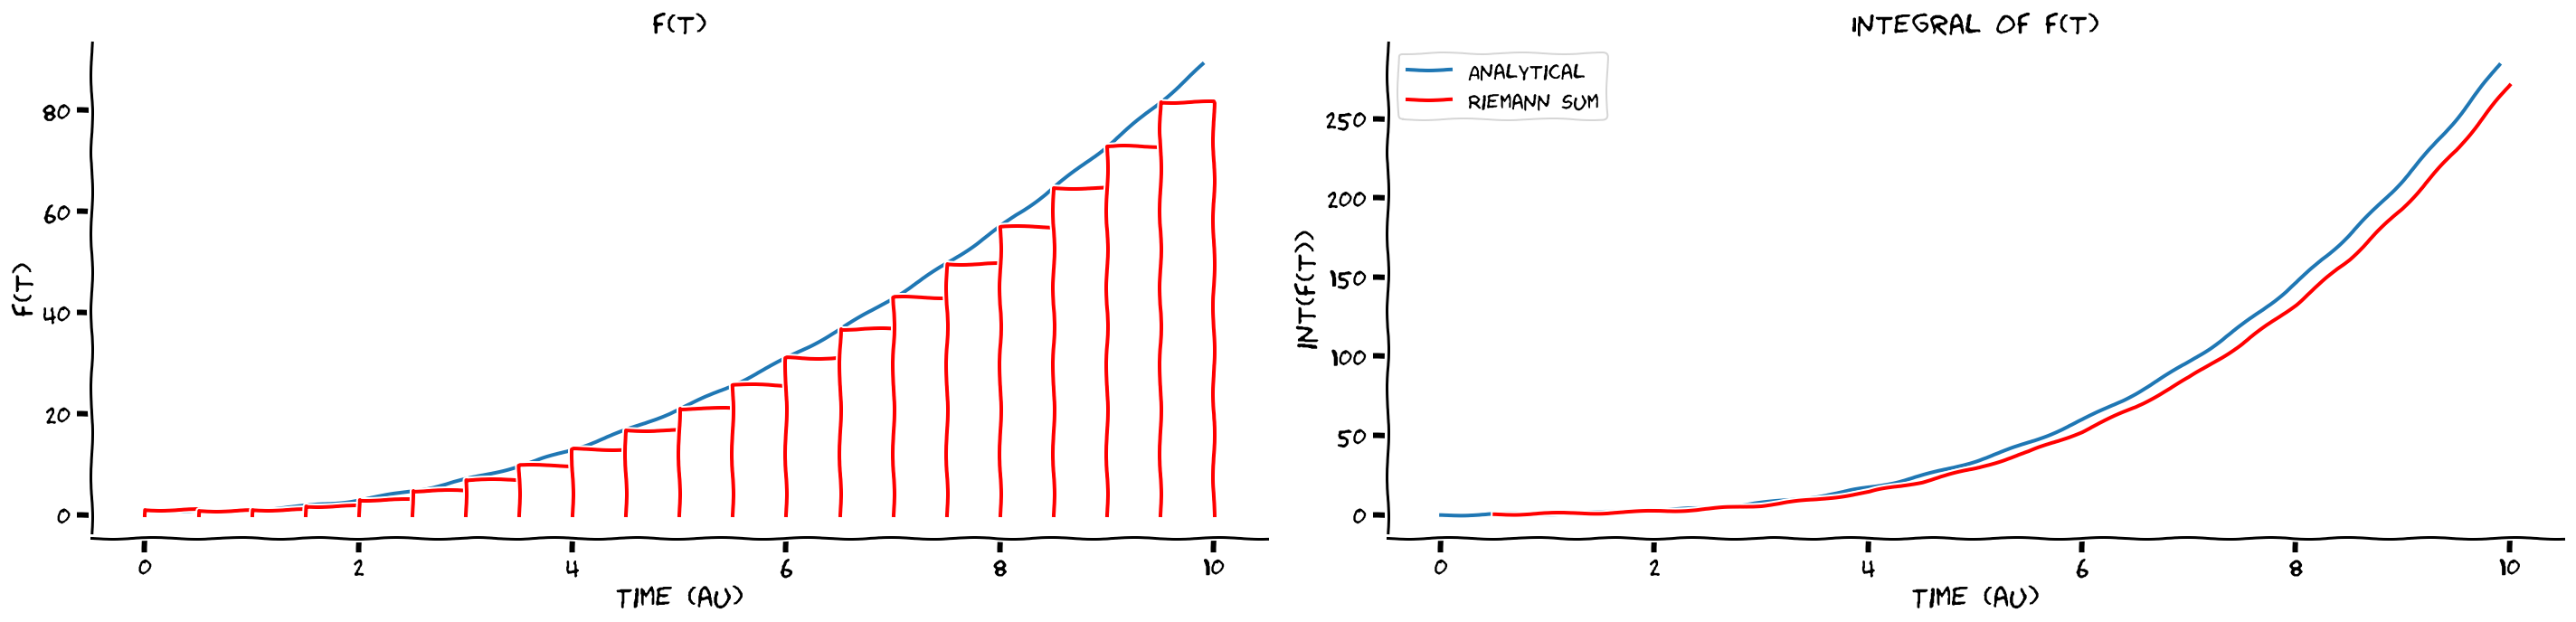
\includegraphics[scale=0.12]{Figures/PreCourse/CFigure4.png}
\end{subbox}


\end{textbox}
%%%%%%%%%%%%%%%%%%%%%%%%%%%%%%%%%%%%%%%%%%%%%%%%%%
%%%%%%%%%%%%%%%%%%%%%%%%%%%%%%%%%%%%%%%%%%%%%%%%%%
\begin{textbox}{Calculus (W0D4T2) - Differential Equations}
%%%%%%%%%%%%%%%
\begin{subbox}{subbox}{Introduction}
\scriptsize
Differential Equations are mathematical equations that describe how something like population or a neuron changes over time. The reason why differential equations are so useful is they can generalise a process such that one equation can be used to describe many different outcomes.
The general form of a first order differential equation is:

\begin{equation}
\frac{d}{dt}y(t) = f\left( t,y(t) \right)
\end{equation}

which can be read as "the change in a process $y$ over time $t$ is a function $f$ of time $t$ and itself $y$".

\end{subbox}
\begin{subbox}{subbox}{Population Differential Equation}
\scriptsize
The linear population equation 
\begin{equation}
\frac{d}{dt}p(t) = \alpha p(t), \, p(0)=P_0
\end{equation}

has the exact solution:$p(t) = P_0 e^{\alpha t}.$
The exact solution written in words is: 
%\begin{equation*}
\begin{align*}
\text{"Population"} &= \text{"grows/declines exponentially as}\\ &\text{ a function of time and birth rate"}.
\end{align*}
\centering
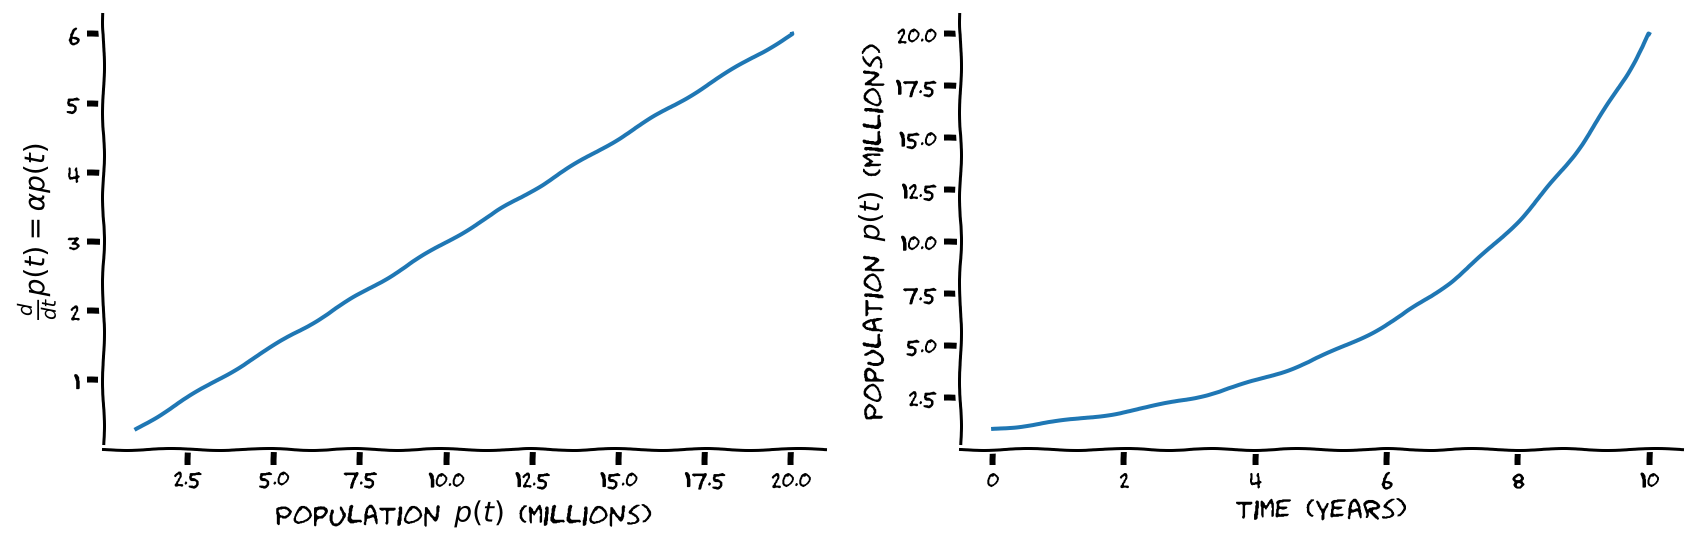
\includegraphics[scale=0.15]{Figures/PreCourse/CFigure5.png}
\end{subbox}
\begin{subbox}{subbox}{The leaky integrate and fire (LIF) model}
\scriptsize
The Leaky Integrate and Fire Model is a linear differential equation that describes the membrane potential ($V$) of a single neuron which was proposed by Louis Édouard Lapicque in 1907.

The subthreshold membrane potential dynamics of a LIF neuron is described by
\begin{align}
\tau_m\frac{dV}{dt} = -(V-E_L) + R_mI\,
\end{align}
where $\tau_m$ is the time constant, $V$ is the membrane potential,  $E_L$ is the resting potential, $R_m$ is membrane resistance, and $I$ is the external input current. 

\centering
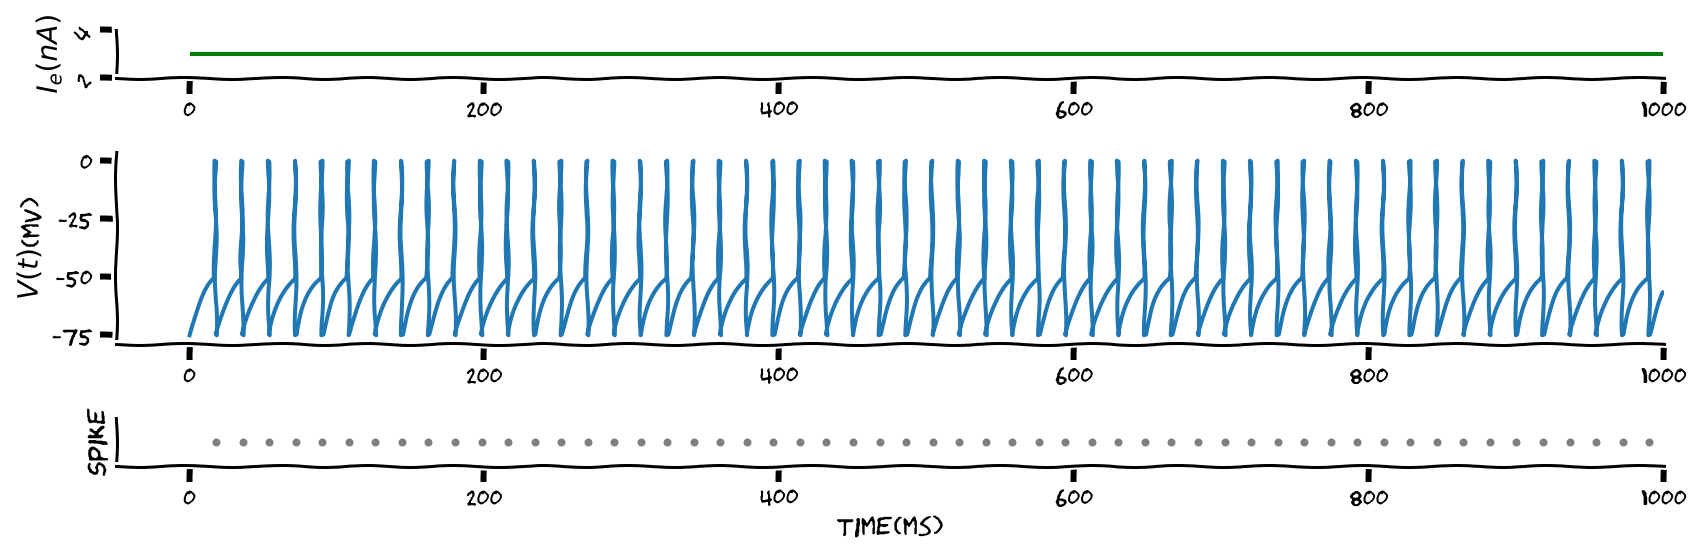
\includegraphics[scale=0.2]{Figures/PreCourse/CFigure6.png}
\end{subbox}
\end{textbox}
%%%%%%%%%%%%%%%%%%%%%%%%%%%%%%%%%%%%%%%%%%%%%%%%%%

%%%%%%%%%%%%%%%%%%%%%%%%%%%%%%%%%%%%%%%%%%%%%%%%%%
%%%%%%%%%%%%%%%%%%%%%%%%%%%%%%%%%%%%%%%%%%%%%%%%%%
\begin{textbox}{Calculus (W0D4T3) - Numerical Methods}
%%%%%%%%%%%%%%%
\begin{subbox}{subbox}{Euler Method}
\scriptsize
The Euler method is one of the straight forward and elegant methods to approximate a differential. It was designed by \href{https://en.wikipedia.org/wiki/Leonhard_Euler}{Leonhard Euler (1707-1783).} 
Simply put we just replace the derivative in the differential equation by the formula for a line and re-arrange.

The slope is the rate of change between two points. The formula for the slope of a line between the points $(t_0,y(t_0))$ and $(t_1,y(t_1))$ is given by:
$$ m=\frac{y(t_1)-y(t_0)}{t_1-t_0}=\frac{\Delta y_0}{\Delta t_0}, $$
where $\Delta y_0=y_1-y_0$ and $\Delta t_0=t_1-t_0$ or in words as
$$ m=\frac{\text{ Change in y} }{\text{Change in t}}. $$
The slope can be used as an approximation of the derivative such that
$$ \frac{d}{dt}y(t)\approx \frac{y(t_0+\Delta t)-y(t_0)}{t_0+\Delta t-t_0}=\frac{y(t_0+dt)-y(t_0)}{\Delta t}$$
where $\Delta t$ is a time-step.
\end{subbox}
\begin{subbox}{subbox}{Population Differential Equation}
\scriptsize
To numerically estimate the population differential equation we replace the derivative with the slope of the line to get the discrete (not continuous) equation where $p_1$ is the estimate of $p(t_1)$. Let $\Delta t=t_1-t_0$ be the time-step and re-arrange the equation gives
\begin{align*}
\color{red}{p_1}&=\color{green}{p_0}+\color{blue}{\Delta t} (\color{blue}{\alpha} \color{green}{p_0} \color{blue}{)}
\end{align*}

where $\color{red}{p_1}$ is the unknown future, $\color{green}{p_0}$ is the known current population, $\color{blue}{\Delta t}$ is the chosen time-step parameter and $\color{blue}{\alpha}$ is the given birth rate parameter.

The solution of the Euler method $p_1$ is an estimate of the exact solution $p(t_1)$ at $t_1$ which means there is a bit of error $e_1$ which gives the equation
\begin{align*}
e_1&=p(t_1)-p_1,\\
\text{Error}&=\text{Exact-Estimate}.
\end{align*}
\centering
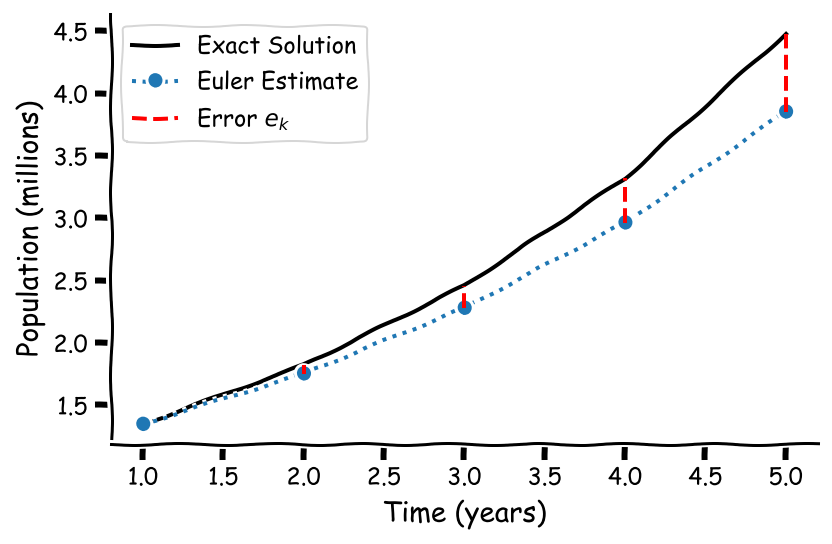
\includegraphics[scale=0.12]{Figures/PreCourse/CFigure7.png}
\end{subbox}

\end{textbox}
%%%%%%%%%%%%%%%%%%%%%%%%%%%%%%%%%%%%%%%%%%%
%%%%%%%%%%%%%%%%%%%%%%%%%%%%%%%%%%%%%%%%%%%
\begin{textbox}{Calculus (W0D4T3) - Numerical Method}
\begin{subbox}{subbox}{Linear Integrate and Fire }
\scriptsize
The solution of the LIF can be estimated by applying the Euler method to give the difference equation:
\begin{align*}
\color{red}{V[k+1]}=\color{green}{V[k]}+\color{blue}{\Delta t}\big(\frac{-(\color{green}{V[k]}-\color{blue}{E_L}) + \color{blue}{R_m}I[k]}{\color{blue}{\tau_m}}\big),\\
\text{for } k=0\cdots n-1,
\end{align*}

where $\color{green}{V[k]}$ is the estimate of the membrane potential at time point $t[k]$,
 $\color{red}{V[k+1]}$ is the unknown membrane potential at $t[k+1]$, $\color{green}{V[k]} $ is known membrane potential, $\color{blue}{E_L}$, $\color{blue}{R_m}$ and $\color{blue}{\tau_m}$ are known parameters, $\color{blue}{\Delta t}$ is a chosen time-step and  $I(t_k)$ is a function for an external input current.
 
\centering
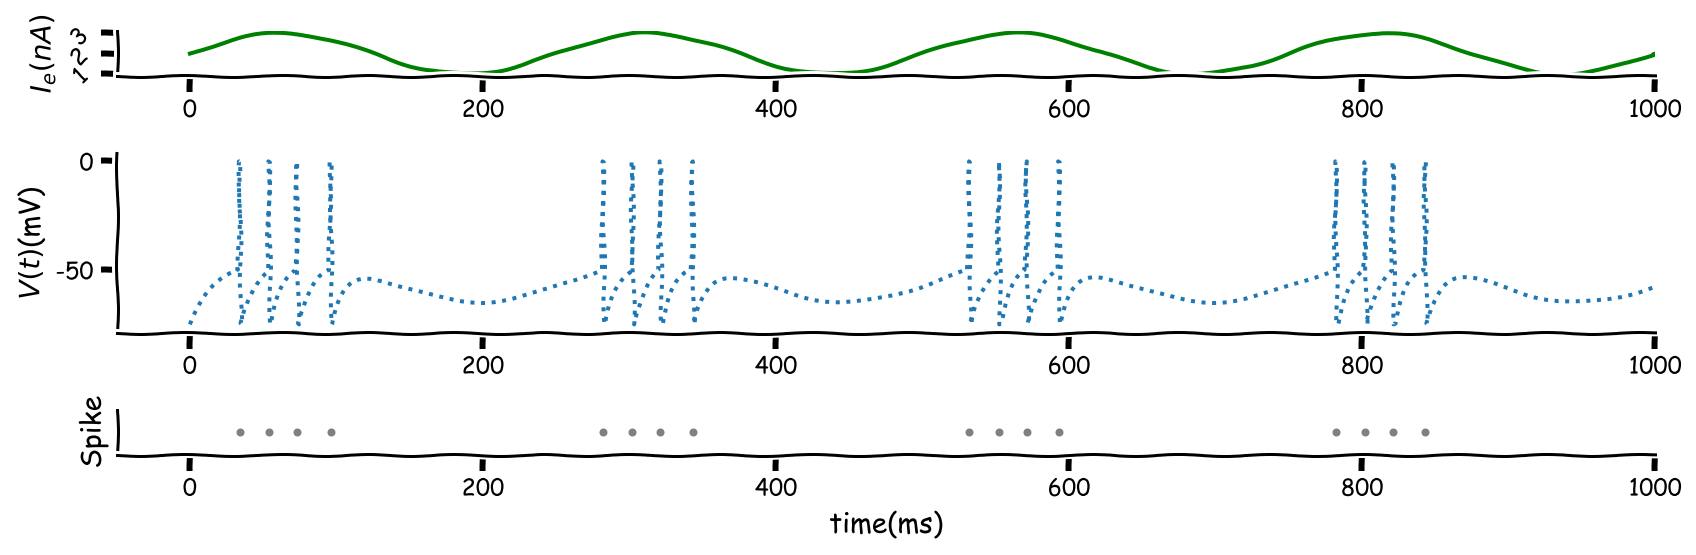
\includegraphics[scale=0.1]{Figures/PreCourse/CFigure8.png}
\end{subbox}

\begin{subbox}{subbox}{Systems of Differential Equations}
\scriptsize
We now model a collection of neurons using a differential equation which describes the firing rate of a population of neurons. 
We will model the firing rate $r$ of two types of populations of neurons which interact, the excitation population firing rate $r_E$ and inhibition population firing rate $r_I$.
 The two coupled differential equations with weights $w$ are:
\begin{align}
\tau_E \frac{dr_E}{dt} &=w_{EE}r_E +w_{EI}r_I, \\
\tau_I \frac{dr_I}{dt} &=w_{IE}r_E +w_{II}r_I ,
\end{align}

The solutions can be approximated using the Euler method such that the equations become:
\begin{align*}
\color{red}{r_E[k+1]}&=\color{green}{r_E[k]}+\color{blue}{\Delta t}\big(\frac{\color{blue}{w_{EE}}\color{green}{r_E[k]}+\color{blue}{w_{EI}}\color{green}{r_I[k]}}{\color{blue}{\tau_E}}\big),\\
\color{red}{r_I[k+1]}&=\color{green}{r_I[k]}+\color{blue}{\Delta t}\big(\frac{\color{blue}{w_{II}}\color{green}{r_I[k]}+\color{blue}{w_{IE}}\color{green}{r_E[k]}}{\color{blue}{\tau_I}}\big),\\
&\text{ for } k=0, \cdots n-1,
\end{align*}
where $r_E[k]$ and $r_I[k]$ are the numerical estimates of the firing rate of the excitation population $r_E(t_k)$ and inhibition population $r_I(t_K)$ and $\Delta t$ is the time-step.

\centering
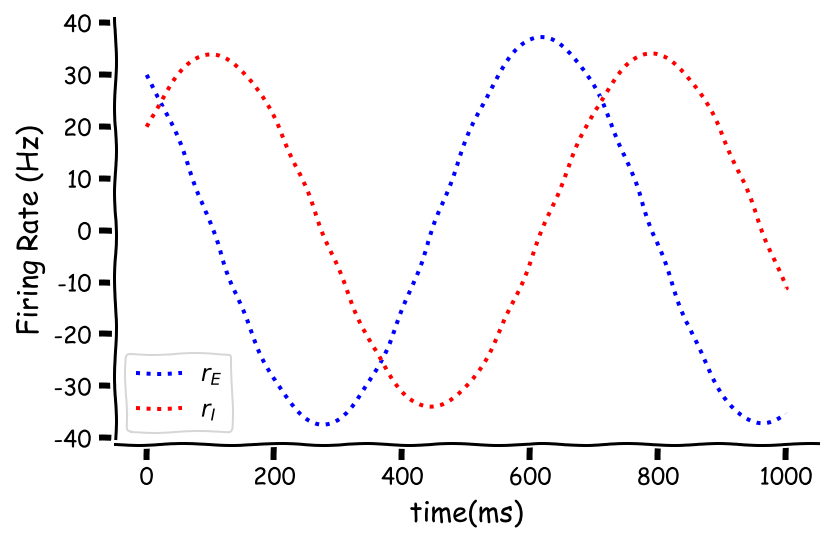
\includegraphics[scale=0.1]{Figures/PreCourse/CFigure9.png}
\end{subbox}
\end{textbox}


\clearpage
\clearpage
\begin{textbox}{\href{https://compneuro.neuromatch.io/tutorials/W0D5_Statistics/student/W0D5_Tutorial1.html}{Statistics (W0D5T1)} - Probability Distributions}
\begin{subbox}{subbox}{Random Walk}
\scriptsize
Stochastic models can be used to create models of behaviour. As an example, imagine that a rat is placed inside a novel environment, a box. We could try and model its exploration behaviour by assuming that for each time step it takes a random uniformly sampled step in any direction (simultaneous random step in x direction and random step in y direction)

\centering
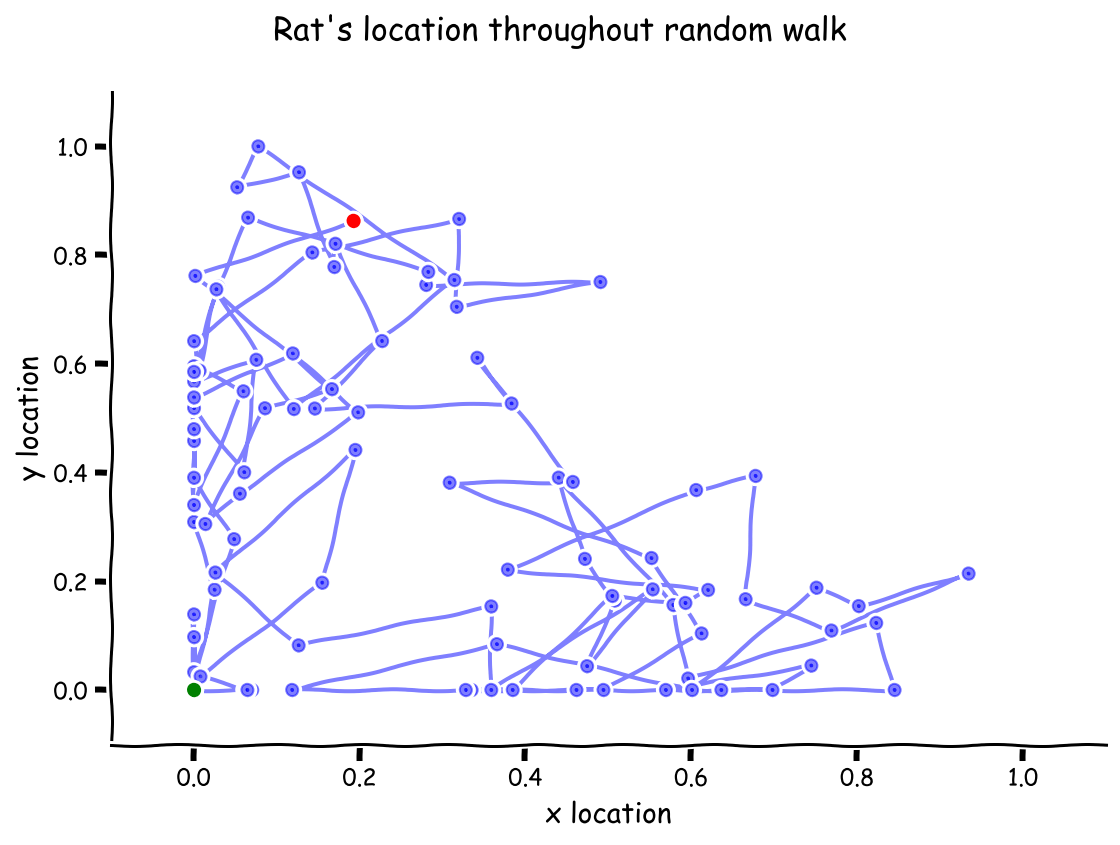
\includegraphics[scale=0.1]{Figures/PreCourse/SFigure1.png}
\end{subbox}

\begin{subbox}{subbox}{Discrete Distributions Differentiation}
\scriptsize{

A simple way to model random behaviour is with a single \textbf{Bernoulli trial}, that has two outcomes, {$Left, Right$}, with probability $P(Left)=p$ and $P(Right)=1-p$ as the two mutually exclusive possibilities (whether the rat goes down the left or right arm of the maze).

\textbf{The binomial distribution} simulates $n$ number of binary events, such as the $Left, Right$ choices of the random rat in the T-maze is given by:
\begin{align}
P(k|n,p) &= \left( \begin{array} \\n \\ k\end{array} \right) p^k (1-p)^{n-k} \\
\binom{n}{k} &= {\frac {n!}{k!(n-k)!}}
\end{align}

where, $p$ is the probability of turning left, $n$ is the number of binary events, or trials, and $k$ is the number of times the rat turned left. The term $\binom {n}{k}$ is the binomial coefficient.

\textbf{The Poisson distribution} is a 'point-process', meaning that it determines the number of discrete 'point', or binary, events that happen within a fixed space or time, allowing for the occurrence of a potentially infinite number of events. The Poisson distribution is specified by a single parameter $\lambda$ that encapsulates the mean number of events that can occur in a single time or space interval.
The formula for a Poisson distribution is: 
\begin{equation}
P(x)=\frac{\lambda^x e^{-\lambda}}{x!}
\end{equation}
where $\lambda$ is a parameter corresponding to the average outcome of $x$.
}
\end{subbox}
\end{textbox}
%%%%%%%%%%%%%%%%%%%%%%%%%%%%%%%%%%%%%%%%%%%%%%%%%
%%%%%%%%%%%%%%%%%%%%%%%%%%%%%%%%%%%%%%%%%%%%%%%%%
\begin{textbox}{\href{https://compneuro.neuromatch.io/tutorials/W0D5_Statistics/student/W0D5_Tutorial1.html}{Statistics (W0D5T1)} - Probability Distributions}
\begin{subbox}{subbox}{Continuous Distributions}
\scriptsize
We do not have to restrict ourselves to only probabilistic models of discrete events. 
While for discrete outcomes we can ask about the probability of an specific event ("what is the probability this neuron will fire 4 times in the next second"), this is not defined for a continuous distribution ("what is the probability of the BOLD signal being exactly 4.000120141..."). Hence we need to focus on intervals when calculating probabilities from a continuous distribution. 

If we want to make predictions about possible outcomes for a continuous distribution we can use the integral
\begin{equation} 
\int_{x_1}^{x_2} P(x) dx 
\end{equation}
where $P(x)$ is a probability density function.

\end{subbox}
\begin{subbox}{subbox}{Gaussian Distribution}
\scriptsize
The most widely used continuous distribution is probably the Gaussian (also known as Normal) distribution. It is extremely common across all kinds of statistical analyses. Because of the central limit theorem, many quantities are Gaussian distributed. Gaussians also have some nice mathematical properties that permit simple closed-form solutions to several important problems. 

The equation for a Gaussian probability density function is:

\begin{equation}
f(x;\mu,\sigma^2) = \mathcal{N}(\mu,\sigma^2) = \frac{1}{\sqrt{2\pi\sigma^2}}\exp\left(\frac{-(x-\mu)^2}{2\sigma^2}\right)
\end{equation}

where $\mu=-1$ is the mean, $\sigma=1$ is the variance and $x$ is the random variable for orientation (degrees). 


\centering
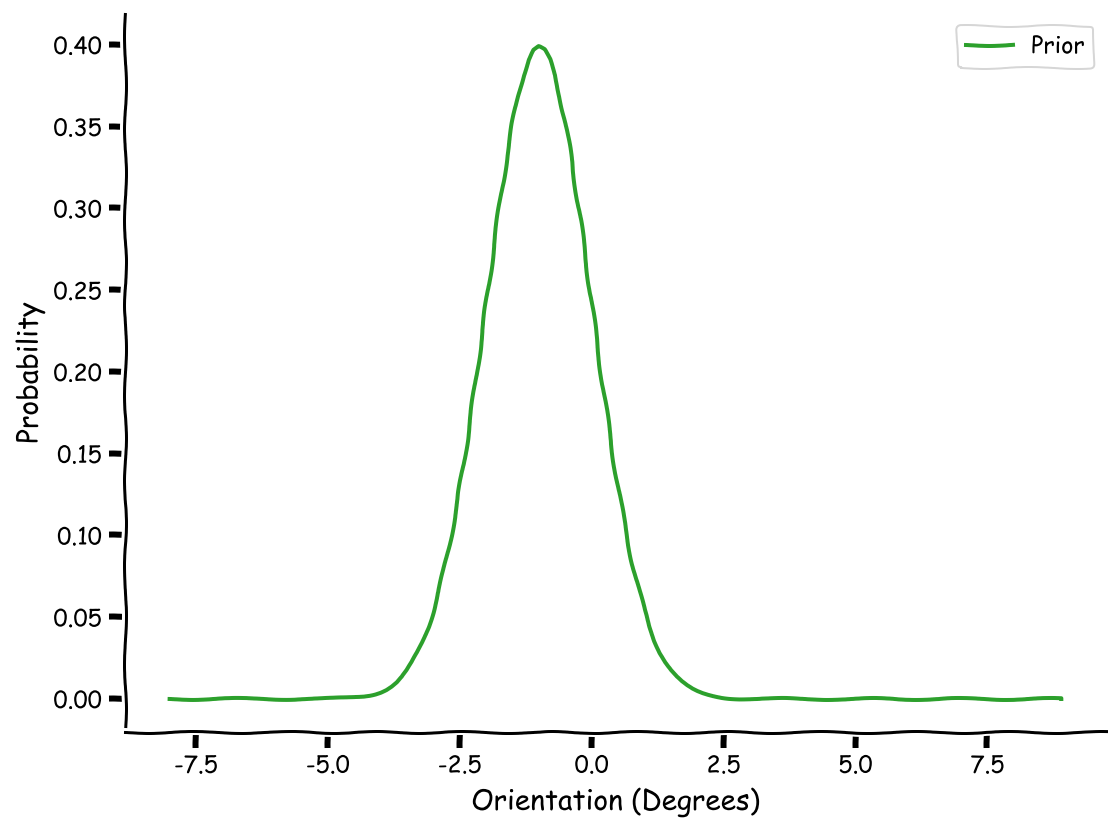
\includegraphics[scale=0.1]{Figures/PreCourse/SFigure2.png}

\end{subbox}
\end{textbox}
%%%%%%%%%%%%%%%%%%%%%%%%%%%%%%%%%%%%%%%%%%%%%%%%%
%%%%%%%%%%%%%%%%%%%%%%%%%%%%%%%%%%%%%%%%%%%%%%%%%
\begin{textbox}{\href{https://compneuro.neuromatch.io/tutorials/W0D5_Statistics/student/W0D5_Tutorial2.html}{Statistics (W0D5T2)} - Statistical Inference}
\begin{subbox}{subbox}{Basic Probability}
\scriptsize

Probability has to be in the range 0 to 1
$P(A) \in  [0,1] $

and the complementary can always be defined as
$$P(\neg A) = 1-P(A).$$
When we have two variables, the \textbf{conditional probability} of $A$ given $B$ is 
$$P (A|B) = P (A \cap B)/P (B)=P (A, B)/P (B)$$
while the \textbf{joint probability} of $A$ and $B$ is
$$P(A \cap B)=P(A,B) = P(B|A)P(A) = P(A|B)P(B) $$
We can then also define the process of \textbf{marginalisation} (for discrete variables) as 
$$P(A)=\sum P(A,B)=\sum P(A|B)P(B)$$ 
where the summation is over the possible values of $B$.

As an example if $B$ is a binary variable that can take values $B+$ or $B0$ then 
$$P(A)=\sum P(A,B)=P(A|B+)P(B+)+ P(A|B0)P(B0). $$

For continuous variables marginalization is given as 
$$P(A)=\int P(A,B) dB=\int P(A|B)P(B) dB.$$ 
\end{subbox}
\begin{subbox}{subbox}{Markov chains}
\scriptsize
The Markov property specifies that you can fully encapsulate the important properties of a system based on its current state at the current time, any previous history does not matter. It is memoryless.

As an example imagine that a rat is able to move freely between 3 areas: a dark rest area
($state=1$), a nesting area ($state=2$) and a bright area for collecting food ($state=3$). Every 5 minutes (timepoint $i$) we record the rat's location. We can use a **categorical distribution** to look at the probability that the rat moves to one state from another.

We can model this as a Markov chain, so the animal is only in one of the states at a time and can transition between the states.
We want to get the probability of each state at time $i+1$.
\begin{align*}
P(state_{i+1} = 1)=&\\ P(state_{i+1}=1|state_i=1)P(state_i = 1)  \\ +P(state_{i+1}=1|state_i=2)P(state_i = 2)  \\ +P(state_{i+1}=1|state_i=3)P(state_i = 3)
\end{align*}

\end{subbox}
\end{textbox}
%%%%%%%%%%%%%%%%%%%%%%%%%%%%%%%%%%%%%%%%%%%%%%%%%
%%%%%%%%%%%%%%%%%%%%%%%%%%%%%%%%%%%%%%%%%%%%%%%%%
\begin{textbox}{\href{https://compneuro.neuromatch.io/tutorials/W0D5_Statistics/student/W0D5_Tutorial2.html}{Statistics (W0D5T2)} - Statistical Inference}
\begin{subbox}{subbox}{Statistical inference and likelihood}
\scriptsize
If we do not know the parameters $\mu$, $\sigma$ that generated the data, we can try to \textbf{infer} which parameter values (given our model) gives the best (highest) likelihood. This is what we call statistical inference: trying to infer what parameters make our observed data the most likely or probable.

A generative model (such as the Gaussian distribution from the previous tutorial) allows us to make predictions about outcomes. 

After we observe $n$ data points, we can evaluate our model (and any of its associated parameters) by calculating the \textbf{likelihood} of our model having generated each of those data points $x_i$.

\begin{equation}
P(x_i|\mu,\sigma)=\mathcal{N}(x_i,\mu,\sigma)
\end{equation}

For all data points $\mathbf{x}=(x_1, x_2, x_3, ...x_n) $ we can then calculate the likelihood for the whole dataset by computing the product of the likelihood for each single data point.

\begin{equation}
P(\mathbf{x}|\mu,\sigma)=\prod_{i=1}^n \mathcal{N}(x_i,\mu,\sigma)
\end{equation}

While the likelihood may be written as a conditional probability ($P(x|\mu,\sigma)$), we refer to it as the \textbf{likelihood function}, $L(\mu,\sigma)$.  This slight switch in notation is to emphasize our focus: we use likelihood functions when the data points $\mathbf{x}$ are fixed and we are focused on the parameters.

Our new notation makes clear that the likelihood $L(\mu,\sigma)$ is a function of $\mu$ and $\sigma$, not of $\mathbf{x}$.


\end{subbox}
\begin{subbox}{subbox}{Maximum likelihood}
\scriptsize
Implicitly, by looking for the parameters that give the highest likelihood in the last section, we have been searching for the \textbf{maximum likelihood} estimate
\begin{equation}
(\hat{\mu},\hat{\sigma}) = \text{argmax}_{\mu,\sigma}L(\mu,\sigma) = \text{argmax}_{\mu,\sigma} \prod_{i=1}^n \mathcal{N}(x_i,\mu,\sigma).
\end{equation}

We want to do inference on this data set, i.e. we want to infer the parameters that most likely gave rise to the data given our model. Intuitively that means that we want as good as possible a fit between the observed data and the probability distribution function with the best inferred parameters. We can search for the best parameters manually by trying out a bunch of possible values of the parameters, computing the likelihoods, and picking the parameters that resulted in the highest likelihood. 

\end{subbox}
\end{textbox}
%%%%%%%%%%%%%%%%%%%%%%%%%%%%%%%%%%%%%%%%%%%%%%%%%
%%%%%%%%%%%%%%%%%%%%%%%%%%%%%%%%%%%%%%%%%%%%%%%%%
\begin{textbox}{\href{https://compneuro.neuromatch.io/tutorials/W0D5_Statistics/student/W0D5_Tutorial2.html}{Statistics (W0D5T2)} - Statistical Inference}
\begin{subbox}{subbox}{Bayesian Inference}
\scriptsize
For Bayesian inference we do not focus on the likelihood function $L(y)=P(x|y)$, but instead focus on the posterior distribution: 

\begin{equation}
P(y|x)=\frac{P(x|y)P(y)}{P(x)}
\end{equation}

which is composed of the **likelihood** function $P(x|y)$, the **prior** $P(y)$ and a normalising term $P(x)$ (which we will ignore for now).

While there are other advantages to using Bayesian inference (such as the ability to derive Bayesian Nets, see optional bonus task below), we will start by focusing on the role of the prior in inference.

\end{subbox}
\begin{subbox}{subbox}{Conjugate priors}
\scriptsize
Bayesian inference can be used for any likelihood distribution, but it is a lot more convenient to work with \textbf{conjugate} priors, where multiplying the prior with the likelihood just provides another instance of the prior distribution with updated values. 

For the binomial likelihood it is convenient to use the beta distribution as a prior

\begin{equation}
f(p;\alpha ,\beta )={\frac {1}{\mathrm {B} (\alpha ,\beta )}}p^{\alpha -1}(1-p)^{\beta -1}
\end{equation}

where $B$ is the beta function, $\alpha$ and $\beta$ are parameters, and $p$ is the probability of the rat turning left or right. The beta distribution is thus a distribution over a probability.

Given a series of Left and Right moves of the rat, we can now estimate the probability that the animal will turn left. Using Bayesian Inference, we use a beta distribution \textbf{prior}, which is then multiplied with the \textbf{likelihood} to create a \textbf{posterior} that is also a beta distribution, but with updated parameters. 

\centering
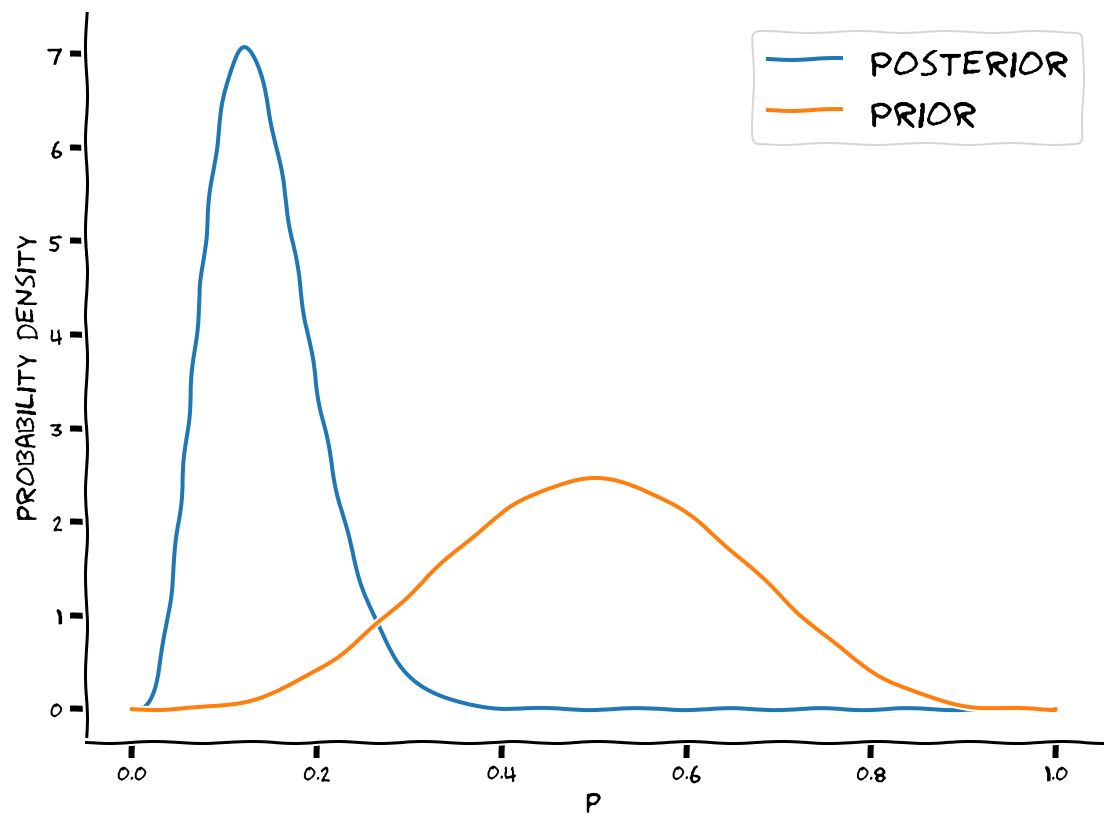
\includegraphics[scale=0.3]{Figures/PreCourse/SFigure3.png}

\end{subbox}
\end{textbox}
\end{multicols}
\end{document}
